%!TeX spellcheck = en-US
% --------------------------------------------------------------
% This is all preamble stuff that you don't have to worry about.
% Head down to where it says "Start here"
% --------------------------------------------------------------

\documentclass[12pt]{article}

\usepackage[margin=.7in]{geometry}
\usepackage{amsmath,amsthm,amssymb}
\usepackage{hyperref} % for external hypertext links
\usepackage{csquotes} % formatting quotes
\usepackage{graphicx} % for images
\graphicspath{ {img/} } % path to im

 %You have to include packages here based on your requiremnts

\begin{document}



% --------------------------------------------------------------
%                         Start here
% --------------------------------------------------------------


\title{Class-Project Proposal}

\author{Optimal Control Theory: EE-5630\\
Name: Joshua Saunders\\}

\maketitle

\hrule
\vspace{5mm}
\textbf{1. Title:}\\

Slot Car Mania - Optimal Control of a Slot Car\\

\textbf{2. Team Members:}\\

This will be a solo project.\\

\textbf{3. Background and Motivation}\\

Connected Autonomous Vehicles (CAVs) are autonomous vehicles that have the
ability to transmit information to other entities and are currently being
researched in the Smart City Lab at CSULA. Currently there is a CSULA senior
design team that is designing an experimental testbed for research into CAVs.
This testbed consists of customized slot cars on a race track shown in Figure
\ref{fig:testbed}.\\

One of the purposes of this testbed is to simulate real-life driving conditions.
Because different classes of drivers are found on the road in the real world
(such as drivers who drive below, at, or above the speed limit) the customized
slot cars should also mimic this driver classes as well. Therefore, this project
will seek to create a class of driver that exceeds the speed limit. The way that
this will be accomplished is by designing a controller such that the slot car
completes a lap of the track from a full stop in the shortest amount of time
as possible.\\

\begin{figure}[H]
    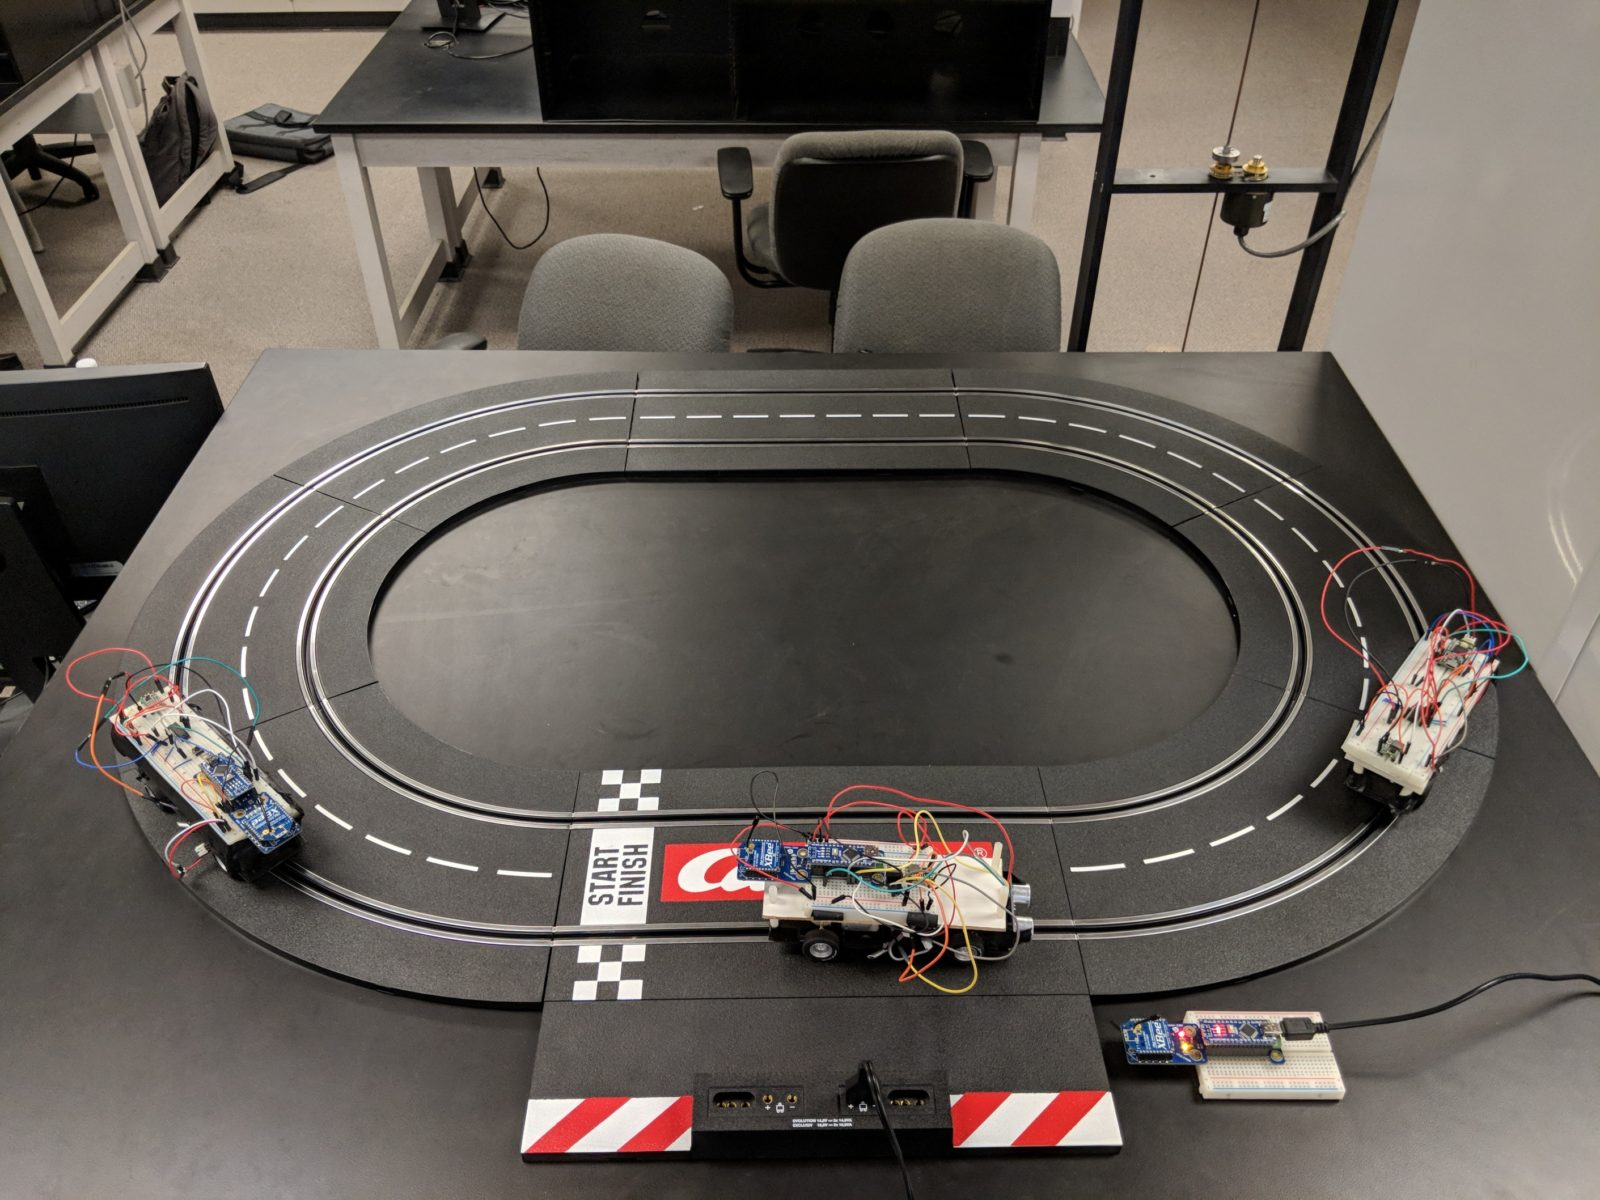
\includegraphics[scale=0.4]{testbed}
    \centering
    \caption{Experimental testbed designed for the Smart City Lab}
    \label{fig:testbed}
\end{figure}

% They are using a
% \href{https://www.carreraslots.com/slot-cars/Digital132124.html}{Carrera slot
% car and track set} to develop this experimental platform. \\


% The University of Maryland's
% Applied Technology and Traffic Analysis Program (ATTAP) \cite{umdcavdef}
% gives three different paradigms of communication that CAVs use
% Vehicle-to-Vehicle (V2V), Vehicle-to-Infrastructure (V2I), and Vehicle to other
% devices (V2X).\\
%
% These communication paradigms allow for a large amount of data to be transmitted
% and, when coupled with the imminent rise of autonomous vehicles, allows for a
% new era in which vehicles can be efficiently routed to their desired locations,
% potentially reduce polution, and potentially reduce the number of
% vehicle-related injuries and fatalities (which, according to \cite{webbnhtsa} is
% a very serious concern). All of this will be accomplished while removing or
% reducing the role of the driver.\\
%
% There are various avenues for research to be conducted with CAVs and in order to
% pursue these avenues . One such
% avenue is to simulate different classes of drivers to more accurately depict
% real-world traffic. For example, anyone who has driven the 110 South freeway
% going through downtown Los Angeles more than once knows that there are many
% different classes of drivers. Such as drivers who go below the speed limit (the
% slow poke), drivers who go the speed limit (the passive driver), and drivers who
% go beyond the speed limit (the speed demon).\\

% In order for research to be pursued in the area of CAVs, an experimental
% platform needs to be developed. Currently there is a CSULA senior design team
% that is designing such an experimental platform. They are using a
% \href{https://www.carreraslots.com/slot-cars/Digital132124.html}{Carrera slot
% car and track set} to develop this experimental platform. \\

% According to the National Highway Traffic Safety Administration (NHTSA)
% \cite{webbnhtsa},
%
% \begin{displayquote}
%   When motor vehicle traffic crashes were ranked within
%   unintentional injury deaths, they were the second leading
%   cause of death during 2015. Among unintentional injury
%   deaths, motor vehicle deaths were the second leading
%   cause for all ages.
% \end{displayquote}

\textbf{4. Description of Systems}\\

The dynamics of the electrical and mechanical parts of the car are

\begin{align}
  L \frac{di(t)}{dt} &= -R i(t) -k_e \omega (t) + u(t) \\
  J \frac{d\omega(t)}{dt} &= -k_t i(t) -b_d \omega (t) + b_s \sin(t)
\end{align}

\noindent where the parameters are described in Table \ref{table:parameters}
below. This system is non-linear, but if the static friction is small enough to
be ignored then the system can become linear.\\

\begin{table}[]
\centering
\caption{Parameter list}
\label{table:parameters}
\begin{tabular}{|c|c|}
 \hline
 \textbf{Parameter} & \textbf{Meaning} \\ \hline
 $i(t)$ & current \\ \hline
 $u(t)$ & voltage \\ \hline
 $\omega(t)$ & angular velocity \\ \hline
 $R$ & resistance \\  \hline
 $L$ & inductance \\ \hline
 $J$ & moment of inertia \\ \hline
 $k_e$ & back emf \\ \hline
 $k_t$ & motor torque \\ \hline
 $b_s$ & static friction \\ \hline
 $b_d$ & dynamic friction \\ \hline
\end{tabular}
\end{table}


\textbf{5. Proposed approach}\\

This is a minimum time problem, therefore the cost function will be \\

\begin{equation}
  J = t_f - t_0
\end{equation}

Most likely a variational approach will be used to solve this problem. Also, I
would like to implement this on a real slot car, time permitting, but most
likely this will be simulated with Python and some external libraries or
Matlab.

\textbf{6. Further Discussion}\\

This problem may end up being too easy so I am aware that it may need to be
modified or scrapped. This is just my proposed starting point. Perhaps a
modification that can be made is to add multiple cars to the track, introduce
constraints such that the cars are to not collide, and have the other cars drive
at a different speed or be human controlled. This will most likely change the
type of problem and thus the cost function and system-level dynamics will need
to be added as well as the dynamics for the car. \\

As a side note, the title is a reference to the
\href{https://youtu.be/HdgVcGjzgR4}{1950 Walt Disney cartoon "Motor Mania"}
starring Goofy.

% \bibliography{bib}
% \bibliographystyle{ieeetr}

% --------------------------------------------------------------
%     You don't have to mess with anything below this line.
% --------------------------------------------------------------

\end{document}
